\documentclass[12pt]{report}
\usepackage{graphicx} % Required for inserting images
\usepackage[a4paper, margin=2.5cm]{geometry}
\graphicspath{{images/}}

\title{CMP5329 Logbook}
\author{Lewis Higgins - Student ID 22133848}
\date{January - March, 2024}


\usepackage[utf8]{inputenc}
\usepackage[T1]{fontenc}
\usepackage{float} % here for H placement parameter
\usepackage{subcaption}

\usepackage{filecontents}
\usepackage[
    firstinits=true, % render first and middle names as initials
    useprefix=true,
    maxcitenames=3,
    maxbibnames=99,
    style=authoryear,
    dashed=false, % re-print recurring author names in bibliography
    natbib=true,
    url=false
]{biblatex}

\renewbibmacro*{volume+number+eid}{%
    \printfield{volume}%
%  \setunit*{\adddot}% DELETED
    \setunit*{\addnbspace}% NEW (optional); there's also \addnbthinspace
    \printfield{number}%
    \setunit{\addcomma\space}%
    \printfield{eid}}
\DeclareFieldFormat[article]{number}{\mkbibparens{#1}}

\addbibresource{logbook.bib}

% Use single quotes around titles:
\usepackage[british]{babel}
\usepackage{csquotes}

\usepackage{hyperref}

\hypersetup{
    colorlinks=true,
    linkcolor=black,
    filecolor=magenta,
    urlcolor=blue,
    citecolor=black,
}


\urlstyle{same}


% To prevent "Chapter N" display for each chapter
\usepackage[compact]{titlesec}
\usepackage{wasysym}
\usepackage{import}

\titlespacing*{\chapter}{0pt}{-2cm}{0.5cm}
\titleformat{\chapter}[display]
{\normalfont\bfseries}{}{0pt}{\Huge}

\newcommand\blfootnote[1]{
    \begingroup
    \renewcommand\thefootnote{}\footnote{#1}
    \addtocounter{footnote}{-1}
    \endgroup
}

\usepackage{fancyhdr}
\usepackage{calc}
\pagestyle{fancy}

\usepackage{tcolorbox}

\setlength\headheight{37pt}

\renewcommand{\chaptermark}[1]{%
    \markboth{#1}{}}

\lhead{Lewis Higgins - ID 22133848~~~~~~~~~~~~~~~
\includegraphics[width=1.75cm]{bcu logo}}
\fancyhead[R]{\leftmark}

\begin{document}

    \pagecolor{yellow}

    \makeatletter
    \begin{titlepage}
        \begin{center}
            
\includegraphics[width=0.7\linewidth]{bcu logo}\\[4ex]
            {\huge \bfseries  \@title }\\[2ex]
            {\huge \bfseries  DRAFT VERSION }\\[2ex]
            {\@author}\\[50ex]
            {\large \@date}
        \end{center}
    \end{titlepage}
    \makeatother
    \thispagestyle{empty}
    \newpage

    \pagecolor{white}

    \tableofcontents
    \chapter*{Introduction}\label{ch:introduction}
    \addcontentsline{toc}{chapter}{Introduction}

    This logbook documents the work completed and knowledge gained across the CMP5329 labs, showcasing
    the use of a wide variety of security techniques and access control methods on a Linux OS\@.
    This logbook specifically covers the following labs:
    \begin{itemize}
        \item Lab 1, covering OpenSSL\@.
        \item Lab 2, covering simple usage of GPG\@.
        \item Lab 5, covering the use of Linux Discretionary Access Control commands.
        \item Lab 6, covering password cracking.
    \end{itemize}

    As per module specifications, screenshots taken in each lab
    include the date and time at which they were taken.\\

    \begin{tcolorbox}[colback=orange!5!white,colframe=orange!75!black,title=Example note]
        Additional notes, such as minor issues encountered or omitted screenshots due to
        work having been done in earlier labs, are documented using these orange notes.
    \end{tcolorbox}

    \begin{tcolorbox}[colback=red!5!white,colframe=red!75!black,title=Example important note]
        Critical issues that required special workarounds are documented using these red notes.
    \end{tcolorbox}


    \chapter{Lab 1 - OpenSSL}\label{ch:lab1}
    \section{Version checking and ciphers}\label{sec:version}

\section{DES symmetric encryption}\label{sec:des}
-a transforms into base64 encoding so that it's "readable" and displayable on a computer screen.
without it, the text will not even be legible, instead showing symbols to represent
non-ASCII/base64?? characters.

\section{AES256 symmetric encryption and decryption}\label{sec:aes256}

\section{Generating \& securing keys}\label{sec:generating-&-securing-keys}
\subsection{RSA private key}\label{subsec:rsa-private-key}

\subsection{Storing DES3 \& passphrase encrypted RSA keys in a file}\label{subsec:storing-keys-in-file}


    \newpage

    \chapter{Lab 2 - Usage of GPG}\label{ch:lab2}
    This lab expanded on the concepts of asymmetric encryption through the use of\newline
GPG/GnuPG (GNU Privacy Guard) to produce, sign and verify public and private keys.

\section{Creating test users}\label{sec:testUsers}
For this lab, two test users were created and used to execute the necessary commands.

\subsection{Elevating the terminal}\label{subsec:sudo}
To add users to the system, administrative privileges are required.
To gain the necessary privileges, the command "sudo -s" or "sudo bash" can be entered
(both commands are functionally identical) which will change the terminal to be at root level.

\begin{figure}[H]
    \centering
    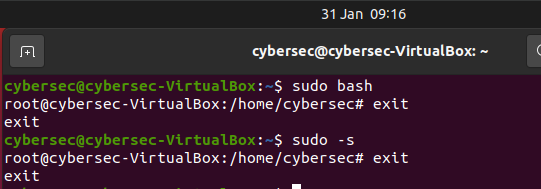
\includegraphics[width=.9\linewidth]{lab2/1}
    \caption{Elevating the terminal.}
    \label{fig:sudo}
\end{figure}

\subsection{Creating Bob and Alice}\label{subsec:createUsers}
With the elevated privileges gained from being a superuser, it is now possible to add users to the system using
"adduser" followed by the given username.
A password will then be necessary, followed by optional information such as phone numbers, which are left empty
for this lab.

\begin{figure}[H]
    \centering
    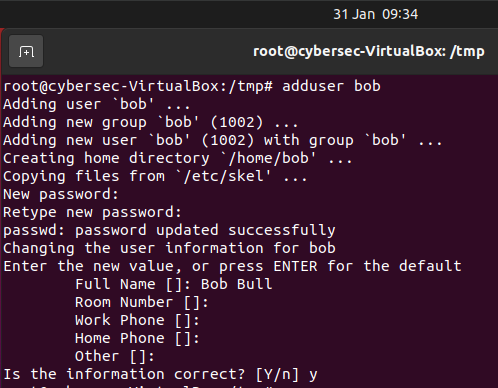
\includegraphics[width=.6\linewidth]{lab2/3}
    \caption{Creating user 'bob'}
    \label{fig:createBob}
\end{figure}

\begin{figure}[H]
    \centering
    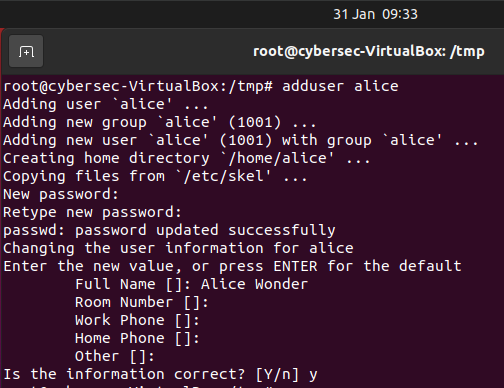
\includegraphics[width=.6\linewidth]{lab2/2}
    \caption{Creating user 'alice'.}
    \label{fig:createAlice}
\end{figure}

For ease of access, multiple terminal tabs can be open at a time, so I elected to use one for the superuser root,
and one each for Bob and Alice.

\begin{figure}[H]
    \centering
    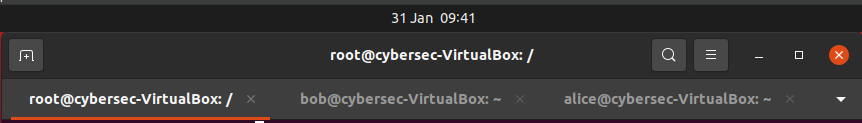
\includegraphics[width=.9\linewidth]{lab2/4}
    \caption{Multiple terminal tabs.}
    \label{fig:terminalTabs}
\end{figure}

I also added these new users to the "sudo" group, allowing them to also use the sudo command to execute commands
with elevated permissions.

\begin{figure}[H]
    \centering
    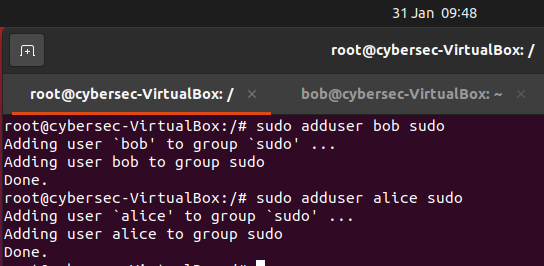
\includegraphics[width=.8\linewidth]{lab2/5}
    \caption{Adding bob and alice to sudo.}
    \label{fig:sudoAdd1}
\end{figure}

\begin{figure}[H]
    \centering
    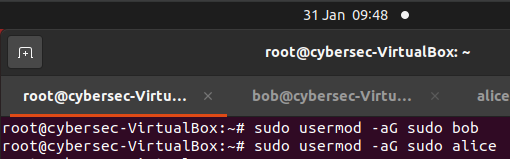
\includegraphics[width=.8\linewidth]{lab2/5b}
    \caption{Adding bob and alice to sudo.}
    \label{fig:sudoAdd2}
\end{figure}

It is possible to switch the active terminal user using the command "su" followed by the account to switch to,
and then the password of the given account.

\begin{figure}[H]
    \centering
    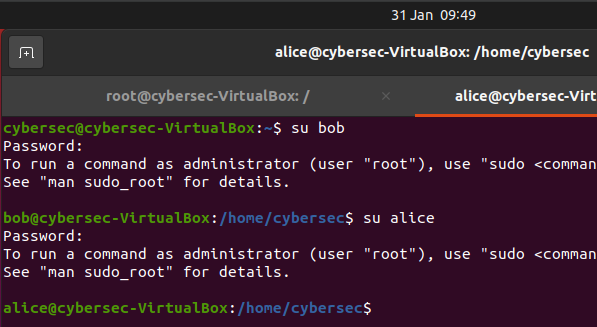
\includegraphics[width=.9\linewidth]{lab2/5c}
    \caption{Switching the active terminal user. Note the prompt about running commands as an administrator,
    which signifies that they were successfully added to the sudo group.}
    \label{fig:suBobAlice}
\end{figure}

\pagebreak

\section{Exchanging files over an insecure channel}\label{sec:tmpExchange}
On standard Linux distributions, the /tmp directory is a public directory accessible to all users.
For this reason, it is therefore unsecure, as every user on the system can access the files placed there.




    \addtocounter{chapter}{2} % Makes the chapter number 5, so sections show as "5.1", "5.1.1"
    \chapter{Lab 5 - Discretionary Access Control}\label{ch:lab5}
    This lab explored the use of Discretionary Access Control methods on a Linux system, which allows
the owner of an object to assign the level of access that other entities will have to said object.

\section{Creating test users and groups}\label{sec:creating-test-users}

\begin{tcolorbox}[colback=orange!5!white,colframe=orange!75!black,title=Note]
    Creating users was already showcased and explained in
    further detail in Lab 2, specifically in figures~\ref{fig:sudo}, \ref{fig:createBob}
    and \ref{fig:sudoAdd1} of section \ref{sec:testUsers}.
\end{tcolorbox}

\noindent For this lab, three test users "Pete", "Ali" and "Mary" were added to the system.
Pete and Ali were assigned to the "Boys" group, whereas Mary was assigned to the "Girls" group.

\subsection{Creating groups}\label{subsec:creating-groups}
With sudo privileges, additional groups can be added to the system.

\begin{figure}[H]
    \centering
    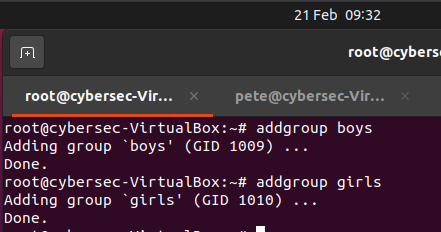
\includegraphics[width=.9\linewidth]{lab5/1}
    \caption{Making the "boys" and "girls" groups.}
    \label{fig:addgroup}
\end{figure}

\subsection{Adding users to groups}\label{subsec:adding-users-to-groups}

The new users were added to the groups mentioned above as well as the sudo group.

\begin{figure}[H]
    \centering
    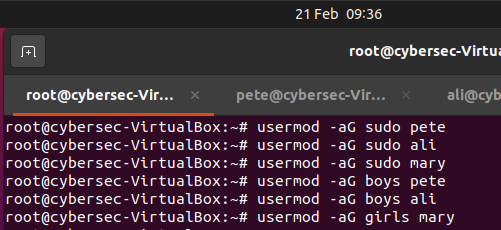
\includegraphics[width=.9\linewidth]{lab5/2}
    \caption{Adding the users to sudo and their respective groups.}
    \label{fig:addToGroup}
\end{figure}

We can verify which groups a given user is in by using the "groups" command.

\begin{figure}[H]
    \centering
    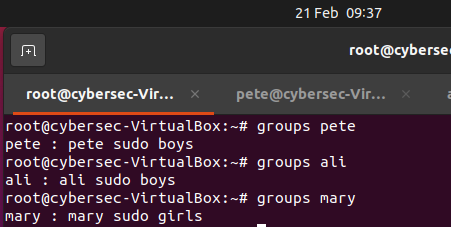
\includegraphics[width=.9\linewidth]{lab5/3}
    \caption{Verifying that the users were added to the groups.}
    \label{fig:checkGroups}
\end{figure}

This can also be checked by viewing all groups on the system via "getent groups".

\begin{figure}[H]
    \centering
    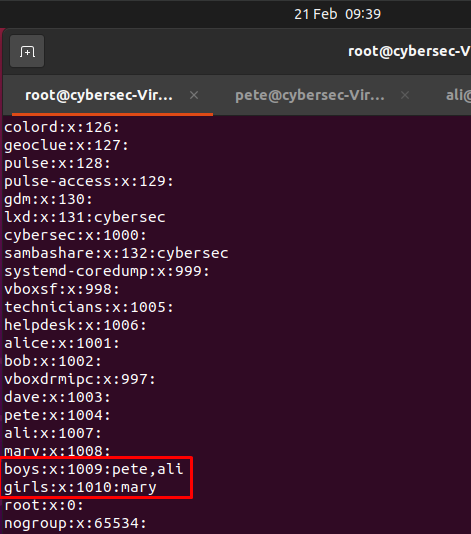
\includegraphics[width=.9\linewidth]{lab5/3b}
    \caption{Seeing all groups (Boys and Girls are highlighted).}
    \label{fig:getent}
\end{figure}

\pagebreak

\section{Using chmod and chgrp to assign permissions}\label{sec:using-chmod}
Chmod changes the permissions for a given file or directory.
It can change permissions for reading, writing and executing files for the owner of the file,
a group of users and other users\footnote{Defined as users that aren't the owner or in an
associated group with permissions.}.
I used \href{https://docs.nersc.gov/filesystems/unix-file-permissions/}{this help page}
\autocite{chmodHelp} to assist in my learning of these commands as well as access control on UNIX
systems.

\subsection{Restricting directory access}\label{subsec:chgrp}
For the purposes of testing, a directory called D1 was added to Mary's home.
This directory was associated with the girls group via chgrp, and modified with a chmod
command so that other users cannot access the directory whatsoever, but Mary and users
of the girls group can read and execute from it.

\begin{figure}[H]
    \centering
    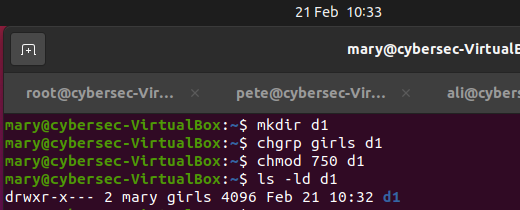
\includegraphics[width=.9\linewidth]{lab5/4}
    \caption{Creating D1 and modifying its permissions.}
    \label{fig:D1}
\end{figure}

\noindent By using the command "ls -ld", the permissions of the directory are outputted.
The returned message reveals that:
\begin{itemize}
    \item The directory owner (Mary) has \textbf{R}ead, \textbf{W}rite and e\textbf{X}ecute permissions.
    \item Group members can \textbf{R}ead and e\textbf{X}ecute.
    \item Others can only e\textbf{X}ecute.
\end{itemize}

This can be tested using Ali and Pete's accounts, which are not members of the
girls group, meaning they are "others".

\begin{figure}[H]
    \centering
    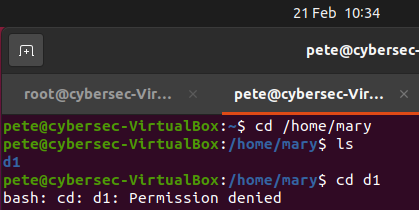
\includegraphics[width=.8\linewidth]{lab5/5}
    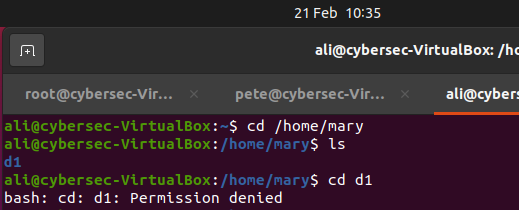
\includegraphics[width=.8\linewidth]{lab5/6}
    \caption{Attempting to access D1 as Pete and Ali.}
    \label{fig:boysD1}
\end{figure}

\begin{tcolorbox}[colback=orange!5!white,colframe=orange!75!black,title=Note]
    An issue arose here that I didn't have another user in the girls group to test access with.
    To fix this, I went back and added the existing Alice account from Lab 2 to the girls group
    with \textit{sudo usermod -aG girls alice}.
\end{tcolorbox}

Using another account in the girls group, we can test if other girls can access the directory,
which succeeds.

\begin{figure}[H]
    \centering
    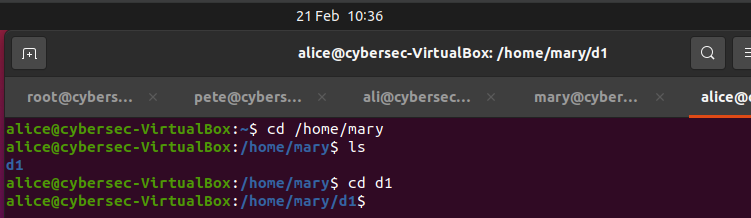
\includegraphics[width=.8\linewidth]{lab5/7}
    \caption{Successfully accessing D1 as Alice.}
    \label{fig:girlsD1}
\end{figure}

Alice is permitted to read the d1 directory and execute files
within it, but she cannot write to it, as intended.

\begin{figure}[H]
    \centering
    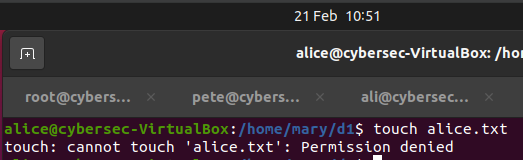
\includegraphics[width=.8\linewidth]{lab5/8}
    \caption{Failing to write to D1 as Alice.}
    \label{fig:girlsWriteD1Fail}
\end{figure}

To test this further, the permissions can then be modified\footnote{770 is "rwxrwx---", which
correlates to the file owner and members of the group having read, write and execute permissions, but other users have none.}
again to allow girls to write files, which will then allow Alice to make the file.

\begin{figure}[H]
    \centering
    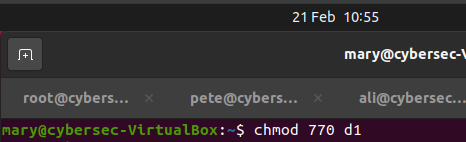
\includegraphics[width=.8\linewidth]{lab5/9}
    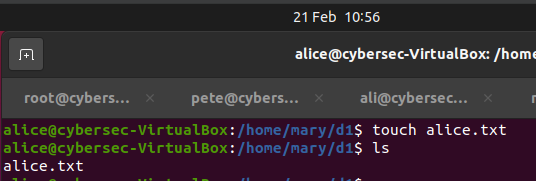
\includegraphics[width=.8\linewidth]{lab5/10}
    \caption{Modifying the permissions of D1, allowing Alice to write the file.}
    \label{fig:girlsWriteD1Success}
\end{figure}

\pagebreak

\subsection{Chgrp and chown}\label{subsec:using-chown}
\begin{tcolorbox}[colback=orange!5!white,colframe=orange!75!black,title=Note]
    I used different directory names ($BoysDirectory$ instead of $Photos$),
    but I have still demonstrated all exercises from this lab.
\end{tcolorbox}
Chown assigns a file or directory's ownership to a specific user.
For this example, we will create a directory in the shared /home folder and assign group ownership
to Boys via chgrp, and using chmod to allow all Boys all permissions, and all other users
read \& execute permissions.

\begin{figure}[H]
    \centering
    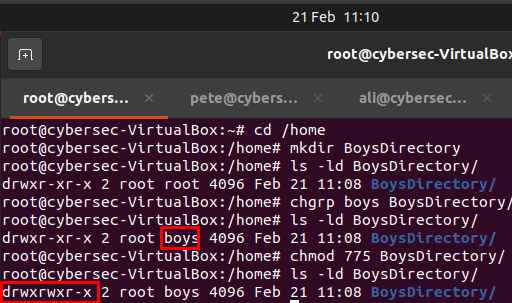
\includegraphics[width=.8\linewidth]{lab5/11}
    \caption{Making BoysDirectory and giving group ownership to Boys.}
    \label{fig:BoysDirectory}
\end{figure}

This new directory can be accessed by all users, but only written to by boys.
We can now test chown by making two subdirectories within BoysDirectory, where one will be owned
by Pete, and one by Ali.
Both users also modify the permissions of their own directories to only be accessible
by them.\footnote{700 is "rwx------", which means only the owner may read,
write and execute.}

\begin{figure}[H]
    \centering
    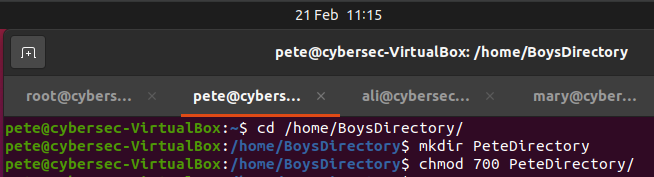
\includegraphics[width=.8\linewidth]{lab5/12}
    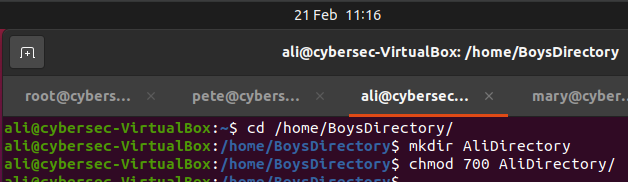
\includegraphics[width=.8\linewidth]{lab5/12b}
    \caption{Creating and modifying each user's directories and access permissions.}
    \label{fig:PeteAliDir}
\end{figure}

\begin{figure}[H]
    \centering
    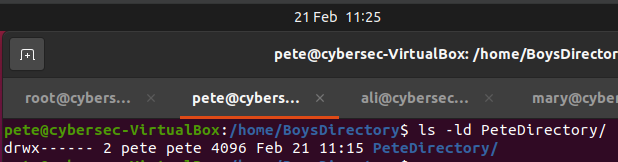
\includegraphics[width=.8\linewidth]{lab5/12c}
    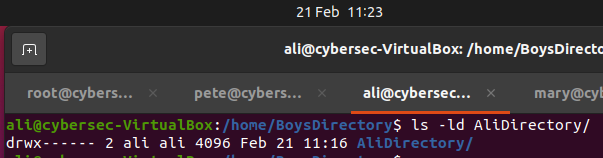
\includegraphics[width=.8\linewidth]{lab5/12d}
    \caption{Viewing the permissions of Pete and Ali's directories.}
    \label{fig:AliDirPerms}
\end{figure}

We can then prove that only the owners of the directories may access them by first accessing their
own directory, but then attempting to access the other user's directory:

\begin{figure}[H]
    \centering
    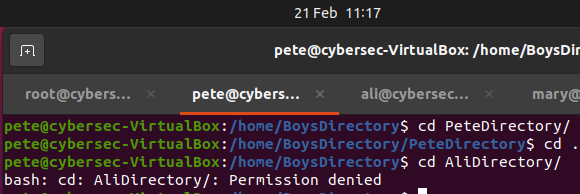
\includegraphics[width=.8\linewidth]{lab5/13}
    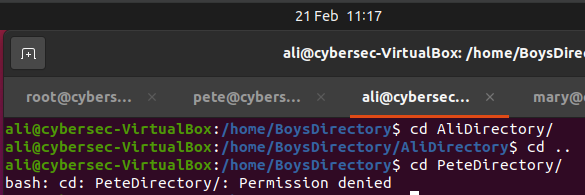
\includegraphics[width=.8\linewidth]{lab5/13b}
    \caption{Successfully accessing their own directory,
        but failing to access the other because the user isn't the owner.}
    \label{fig:PeteAliDirFail}
\end{figure}

An important distinction to be made here is that these subdirectories are owned by Pete and
Ali respectively.
They do \textbf{not} inherit the boys group ownership by default, meaning that commands to
change group permissions will be ineffective for other boys, as everyone who is not the owner
is considered "other" unless chgrp is used, as seen in Figure \ref{fig:PeteAliDirFail}.

\begin{figure}[H]
    \centering
    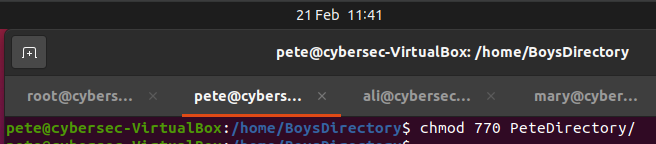
\includegraphics[width=.8\linewidth]{lab5/14}
    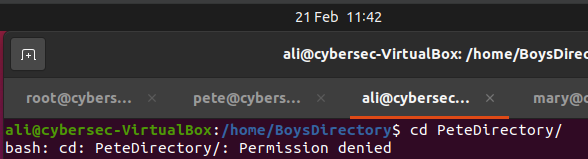
\includegraphics[width=.8\linewidth]{lab5/14b}
    \caption{Giving group RWX access to PeteDirectory}
    \label{fig:PeteDirFail}
\end{figure}

Ali still can't access the directory because he is not part of the "Pete" group, but he
(and any other users) would be able to use permissions given to "others".









    \chapter{Lab 6 - Password Cracking}\label{ch:lab6n}
    In this lab, a simple brute-force attack program written in C was used to crack a hashed account password.

\section{Linux password storage}\label{sec:linux-password-storage}
Linux systems store user account details across two files, $/etc/passwd$ and $/etc/shadow$.
I learned information about this from
\href{https://www.cyberciti.biz/faq/understanding-etcpasswd-file-format/}{this site}~\autocite{accStorage},
which states that the public unencrypted ASCII file $/etc/passwd$ contains a line for each user on the system,
with publicly accessible information such as username, user ID and group ID, whereas the encrypted $/etc/shadow$
file contains the encrypted passwords of users on the system.

\begin{figure}[H]
    \centering
    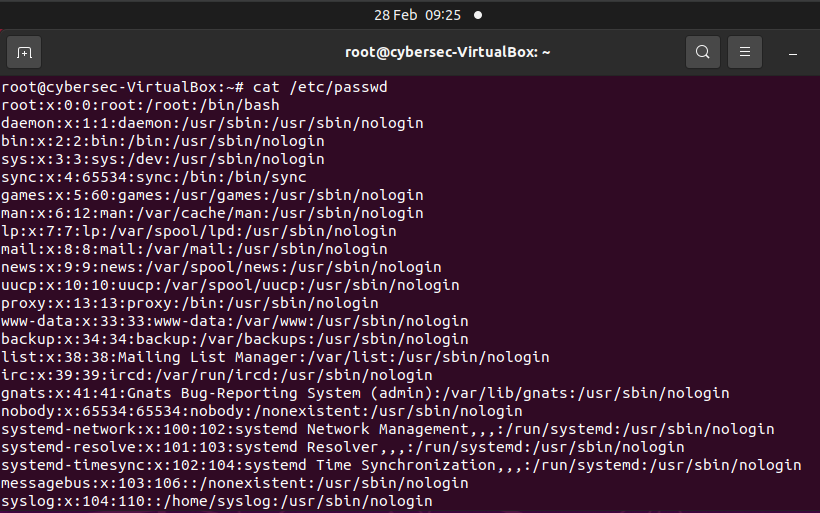
\includegraphics[width=.9\linewidth]{lab6/1}
    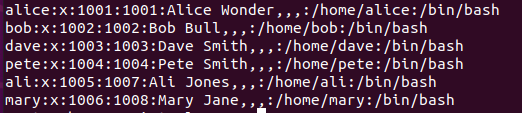
\includegraphics[width=.9\linewidth]{lab6/1b}
    \caption{Some of the contents of /etc/passwd, with the created users from earlier labs.}
    \label{fig:etcpasswd}
\end{figure}

\begin{figure}[H]
    \centering
    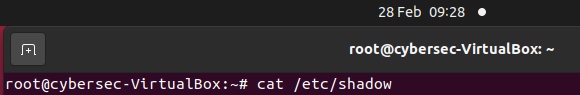
\includegraphics[width=.9\linewidth]{lab6/2}
    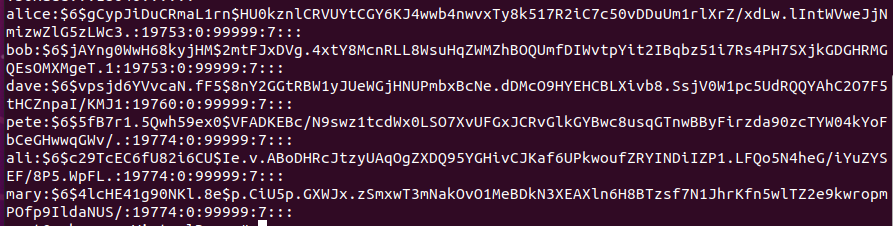
\includegraphics[width=.9\linewidth]{lab6/2b}
    \caption{Some of the contents of /etc/shadow, with the created users from earlier labs.}
    \label{fig:etcshadow}
\end{figure}



%\begin{itemize}
%    \item Username
%    \item Password - This doesn't store the actual password, which is located in $/etc/shadow$, but rather
%          an "x", indicative of if their encrypted and salted password is in the shadow file.
%    \item User ID
%    \item Primary group ID
%    \item User ID info - Comments such as their full name.
%    \item Home directory
%    \item The user's shell
%\end{itemize}



\section{crack.c}\label{sec:crack.c}
The provided code in crack.c is a small program that performs a dictionary attack,
cracking hashed passwords by hashing each word in the dictionary, adding the salt
and comparing the product to the hashed password.
The Ubuntu dictionary is located in $/usr/share/dict/words$.

\subsection{Importing and compilation}\label{subsec:importing-and-compilation}
First, this code must be ported into the Ubuntu VM using "nano crack.c", and pasting the code from Moodle.

\begin{figure}[H]
    \centering
    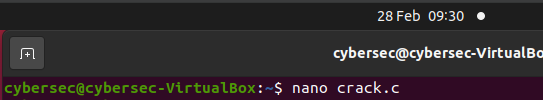
\includegraphics[width=.9\linewidth]{lab6/3}
    \caption{Porting crack.c into the VM.}
    \label{fig:nanoCrackC}
\end{figure}

\begin{figure}[H]
    \centering
    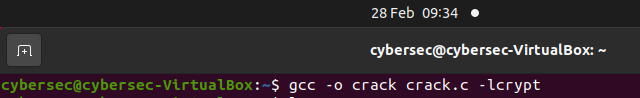
\includegraphics[width=.9\linewidth]{lab6/3b}
    \caption{Compiling crack.c.}
    \label{fig:compile}
\end{figure}

The '-lcrypt' argument supplies the Linux crypt library when compiling, allowing the crypt() function
to be used more securely.

\pagebreak

\subsection{Creating a test user}\label{subsec:creating-a-test-user}
To use the program, it will be necessary to create a new user, whose password can be found in the dictionary.
For this, the user 'fred' will be created, and his password will be 'peach'.
We can see if 'peach' appears in the dictionary, as well as the overall dictionary word count.

\begin{figure}[H]
    \centering
    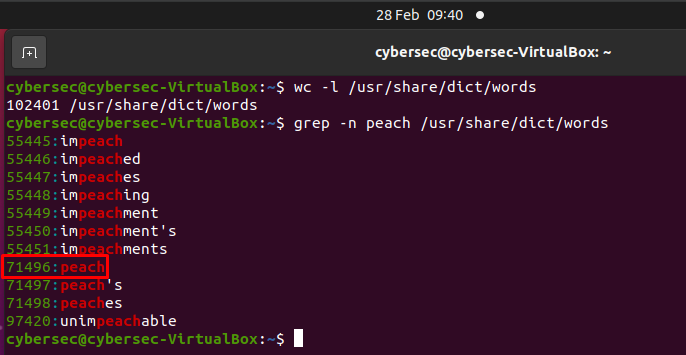
\includegraphics[width=.9\linewidth]{lab6/4}
    \caption{Checking the dictionary for the word 'peach', which is the 71496th entry.}
    \label{fig:checkDict}
\end{figure}

\begin{figure}[H]
    \centering
    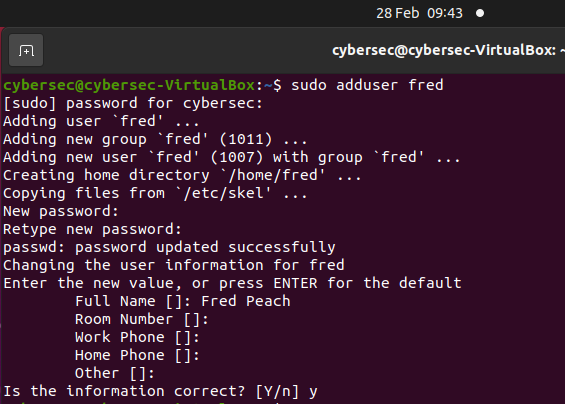
\includegraphics[width=.6\linewidth]{lab6/4b}
    \caption{Creating the 'fred' user, with the password 'peach'.}
    \label{fig:createFred}
\end{figure}

It will then be necessary to get the hashed version of Fred's password, which can be done using
"\textbf{cat /etc/shadow | grep fred | awk -F: '\{ print \$2 \}'}".
This command will read the shadow file, selecting the row starting with 'fred'.
Then, it will extract his hash by selecting the second column.

\begin{figure}[H]
    \centering
    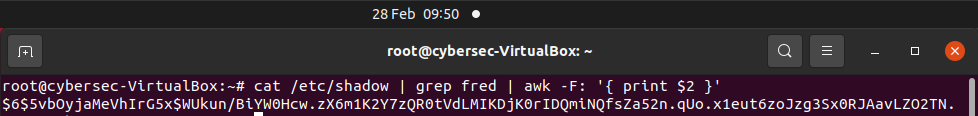
\includegraphics[width=.9\linewidth]{lab6/5}
    \caption{Viewing fred's hashed password.}
    \label{fig:viewFredHash}
\end{figure}

\subsection{Cracking the password}\label{subsec:cracking-the-password}
The program takes two arguments, with the first being the salt used on the password and the
second being the entire hashed password.
It requires the salt as an argument because it will apply the salt to each password it checks.
As seen in Figure \ref{fig:viewFredHash}, Fred's entire hashed password is

\begin{verbatim}
$6$5vbOyjaMeVhIrG5x$WUkun/BiYW0Hcw.zX6m1K2Y7zQR0tVdLMIKDjK0rIDQmiNQfsZa
52n.qUo.x1eut6zoJzg3Sx0RJAavLZO2TN.
\end{verbatim}

We can figure out the salt used on this password by looking at how it starts.
The first 20 characters of this password are the salt, noticeable by how they are between two dollar signs.
This can be supplied as the first argument for the compiled crack program, and the second argument would be the
entire password, including the salt as well.
Ultimately, this forms the following command:

\begin{verbatim}
./crack '$6$5vbOyjaMeVhIrG5x$'
'$6$5vbOyjaMeVhIrG5x$WUkun/BiYW0Hcw.zX6m1K2Y7zQR0tVdLMIKDjK0rIDQmiNQfsZa
52n.qUo.x1eut6zoJzg3Sx0RJAavLZO2TN.'
\end{verbatim}

It is imperative to use \textbf{quotation} marks rather than speech marks, as Linux will otherwise incorrectly
interpret the arguments given due to there being dollar signs in the hash, meaning that the crack will be
unsuccessful.

\begin{figure}[H]
    \centering
    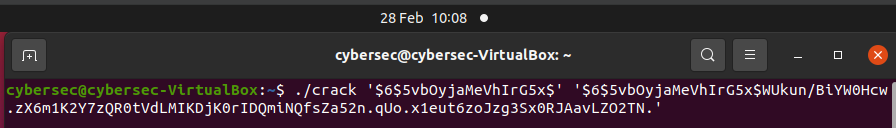
\includegraphics[width=\linewidth]{lab6/6}
    \caption{Entering the command.}
    \label{fig:cracking}
\end{figure}

\begin{figure}[H]
    \centering
    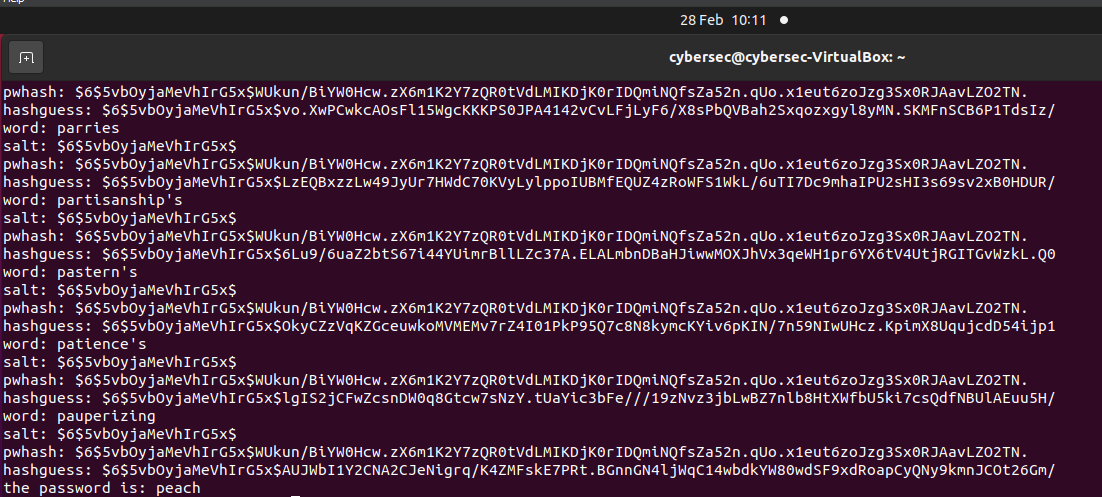
\includegraphics[width=.9\linewidth]{lab6/6b}
    \caption{The hashed password is revealed as 'peach'.}
    \label{fig:cracked}
\end{figure}

Note the differing timestamps, showing how this took around 3 minutes to execute.
This is because the word 'peach' occurs so late in the dictionary as seen in Figure \ref{fig:checkDict}.




    \chapter*{Conclusion}\label{ch:conclusion}
    \addcontentsline{toc}{chapter}{Conclusion}

    \large\textbf{Remember to change the title page to not be yellow!}

    Check Lab2 Sec \ref{subsec:sudo}, is sudo -s actually the same?
    Also in Figure \ref{fig:sudoAdd1}, both of those are the same.

    \noindent Looking at your header, specifically in Lab 5 as well, it may be worth
    removing the "Lab 1 -" "Lab 2 -" parts of the chapter names as you already did it
    using chapter numbering.


    \large\textbf{You've not done what Lab 5 asks you to. Yes, you've demonstrated the knowledge,
    but it's not in the specific way they wanted. Redo it with the /home/photos folder. Could just
    mv it for rename but timestamps may snitch?}

    \printbibliography

\end{document}